\documentclass{article}
\usepackage[utf8]{inputenc}
\usepackage{array}
\usepackage{multirow}
\usepackage{graphicx}
\usepackage{color}   %May be necessary if you want to color links
\usepackage{hyperref}
\usepackage{longtable}
\usepackage{float}
\usepackage[table]{xcolor}
\usepackage{amssymb}
\usepackage{minted}
\setlength{\arrayrulewidth}{0.5mm}
\setlength{\tabcolsep}{18pt}
\renewcommand{\arraystretch}{2.5}
\hypersetup{
    colorlinks=false, %set true if you want colored links
    linktoc=all,     %set to all if you want both sections and subsections linked
    %linkcolor=blue,  %choose some color if you want links to stand out
}

\title{DREAM - DD}
\author{Filippo Lazzati}
%\date{October 2021}

\begin{document}
\thispagestyle{empty} 
\begin{titlepage}
    \begin{center}
       %\vspace*{2cm}
       {\Huge \textbf{DREAM}} %%Replace this with the Title of your research
       \vspace{0.5cm}
       \\
    \begin{LARGE}
        {Data-dRiven PrEdictive FArMing in Telangana}
        \vspace{1.0cm}
        \\
        {\textit{Design Document - DD}}
        
\includegraphics[width=13cm]{logo/polimi.png}
       \vspace{1.5cm}
        
        {Christian Grasso - Filippo Lazzati - Chiara Magri}
       \vspace{0.5cm}
       {Year: 2021/2022}
       
    \end{LARGE}  
   \end{center}
\end{titlepage}
\newpage
\tableofcontents %this command creates an index
\newpage

\section{Introduction}
A DD\footnote{Design Document. See section \ref{Abbreviations}}, according to the definition provided by the \textbf{IEEE Std 1016™-2009} standard, is \textit{a representation of a software design that is to be used for recording design information, addressing various design concerns, and communicating that information to the design’s stakeholders}. It should be noticed that, in this document, instead of using the abbreviation SDD, which stands for "Software Design Description", is used DD. In other words, a DD is a document that is used by \textit{acquirers, project managers, quality assurance staff, configuration managers, software designers, programmers, testers, and maintainers} to retrieve the specific design information needed by the specific stakeholder.
\subsection{Purpose}\label{Purpose}
\verb|DREAM|, the system to-be, aims to help policy makers 
formulating policies in the field of agriculture.  Moreover, \verb|DREAM| aims to help farmers by putting them in contact with each other so that they can exchange advice and aids. Finally, \verb|DREAM| also schedules the daily work of agronomists and make them visit the worse-performing farmers. These are the main goals of \verb|DREAM| which shall be data-driven, namely it shall intensively exploits data to perform the tasks it is asked to do. The requirements that allow the system to satisfy the goals as well as a detailed list of all the goals are present respectively in \textit{RASD - 3.2 Functional requirements} and in \textit{RASD - 1.1 Purpose}. In this document the focus in on the design, that is on the description of the components and the interaction among them and with external systems through interfaces which compose the system and allow the satisfaction of the requirements and, at the end, of the goals.
\subsection{Scope}
The system to-be has three major stakeholders: the policy makers, the agronomists and the farmers. The needs that \verb|DREAM| aims to satisfy differ among them, and the main goals of the system have been identified in section\ref{Purpose}. For a detailed description and explanation of the context in which \verb|DREAM| operates the reader should refer to the \textit{RASD - 1.2 Scope} section. In here, we briefly tell about the main design concerns of such stakeholders.\\
First of all, all of them have goals that, in order to be satisfied, require the storage of a large volume of data (after all, \verb|DREAM| is a data-driven system), and therefore scalable technologies suitable to manage the required amount of information have to be used. Furthermore, the stakeholders are not assumed to be expert in computer science, thus a graphical interface is needed; more specifically, the idea is to implement a web application to facilitate the access to the system to all the users and from any kind of device (computer, smartphone, ...).
\subsection{Definitions, Acronyms, Abbreviations}\label{Abbreviations}
This section provides a list of the main abbreviations, acronyms and definitions adopted in the document:
\begin{itemize}
    \item Design Document (DD): "An SDD is a representation of a software design to be used for communicating design information to its stakeholders. The requirements for the design languages (notations and other representational schemes) to be used for conformant SDDs are specified.
This standard is applicable to automated databases and design description languages but can be
used for paper documents and other means of descriptions".
\end{itemize}
\subsection{Revision history}
\raggedright
\begin{tabular}{ |c | c |}
\hline
 \textit{revision} & \textit{changes} \\ 
 \hline
 1.0 &  initial version\\ 
 \hline
\end{tabular}
\subsection{Reference Documents}
\begin{itemize}
    \item \textit{IEEE Std 1016™-2009}, the standard for information technology, systems design, Software Design Descriptions. It describes the "required information content and organization for software design descriptions (SDDs)";
    \item \textit{ISO/IEC/IEEE 42010}, the standard for architecture description in systems and software engineering, that "addresses the creation, analysis and sustainment of architectures of systems
through the use of architecture descriptions".
\end{itemize}
\subsection{Document Structure}
This document complies with the SDD\footnote{Software Design Descriptions} standard structure as it is defined in the \textit{IEEE Std 1016™-2009}, sections 4 and 5. Nevertheless, the contents have been ordered in a way that best fits the specific topics of this document and to facilitate the readers in the reading of this DD\footnote{Design Document.}.
The document is divided in 5 main parts:
\begin{enumerate}
\item the first part (to which this section belongs) provides an introduction to the system to-be, \verb|DREAM|, helping in the reading of the following sections;
\item the second part provides the out-and-out design decisions under which \verb|DREAM| is implemented. This part contains UML\footnote{Unified Modeling Language.} diagrams as well as text descriptions of the components of the system along with their interfaces, and explanations of the selected architectural styles and design patterns and possible other design decisions;
\item the third part describes the user interface. This part is a continuation of the \textit{RASD - 3.1.1 User Interfaces} section, which enters the details of the design choices;
\item the fourth part shows how the requirements identified in the \textit{RASD - 3.2 Functional requirements} section have brought to the introduction of a specific component/interface in the system;
\item the fifth and last part is about a plan to follow for the implementation of the system, namely from which subcomponent to start, which subcomponents can be implemented in parallel, and about a plan for the integration of such subcomponents and also a plan for testing the integration.
\end{enumerate}
It should be remarked that the structure of this document does not follow a logic or temporal order, but whoever is interested in the reading can jump from a section to another, because the purpose of it is to be a reference document.
\section{Architectural design}
\subsection{Overview}
\subsection{Component view}\label{Component view}
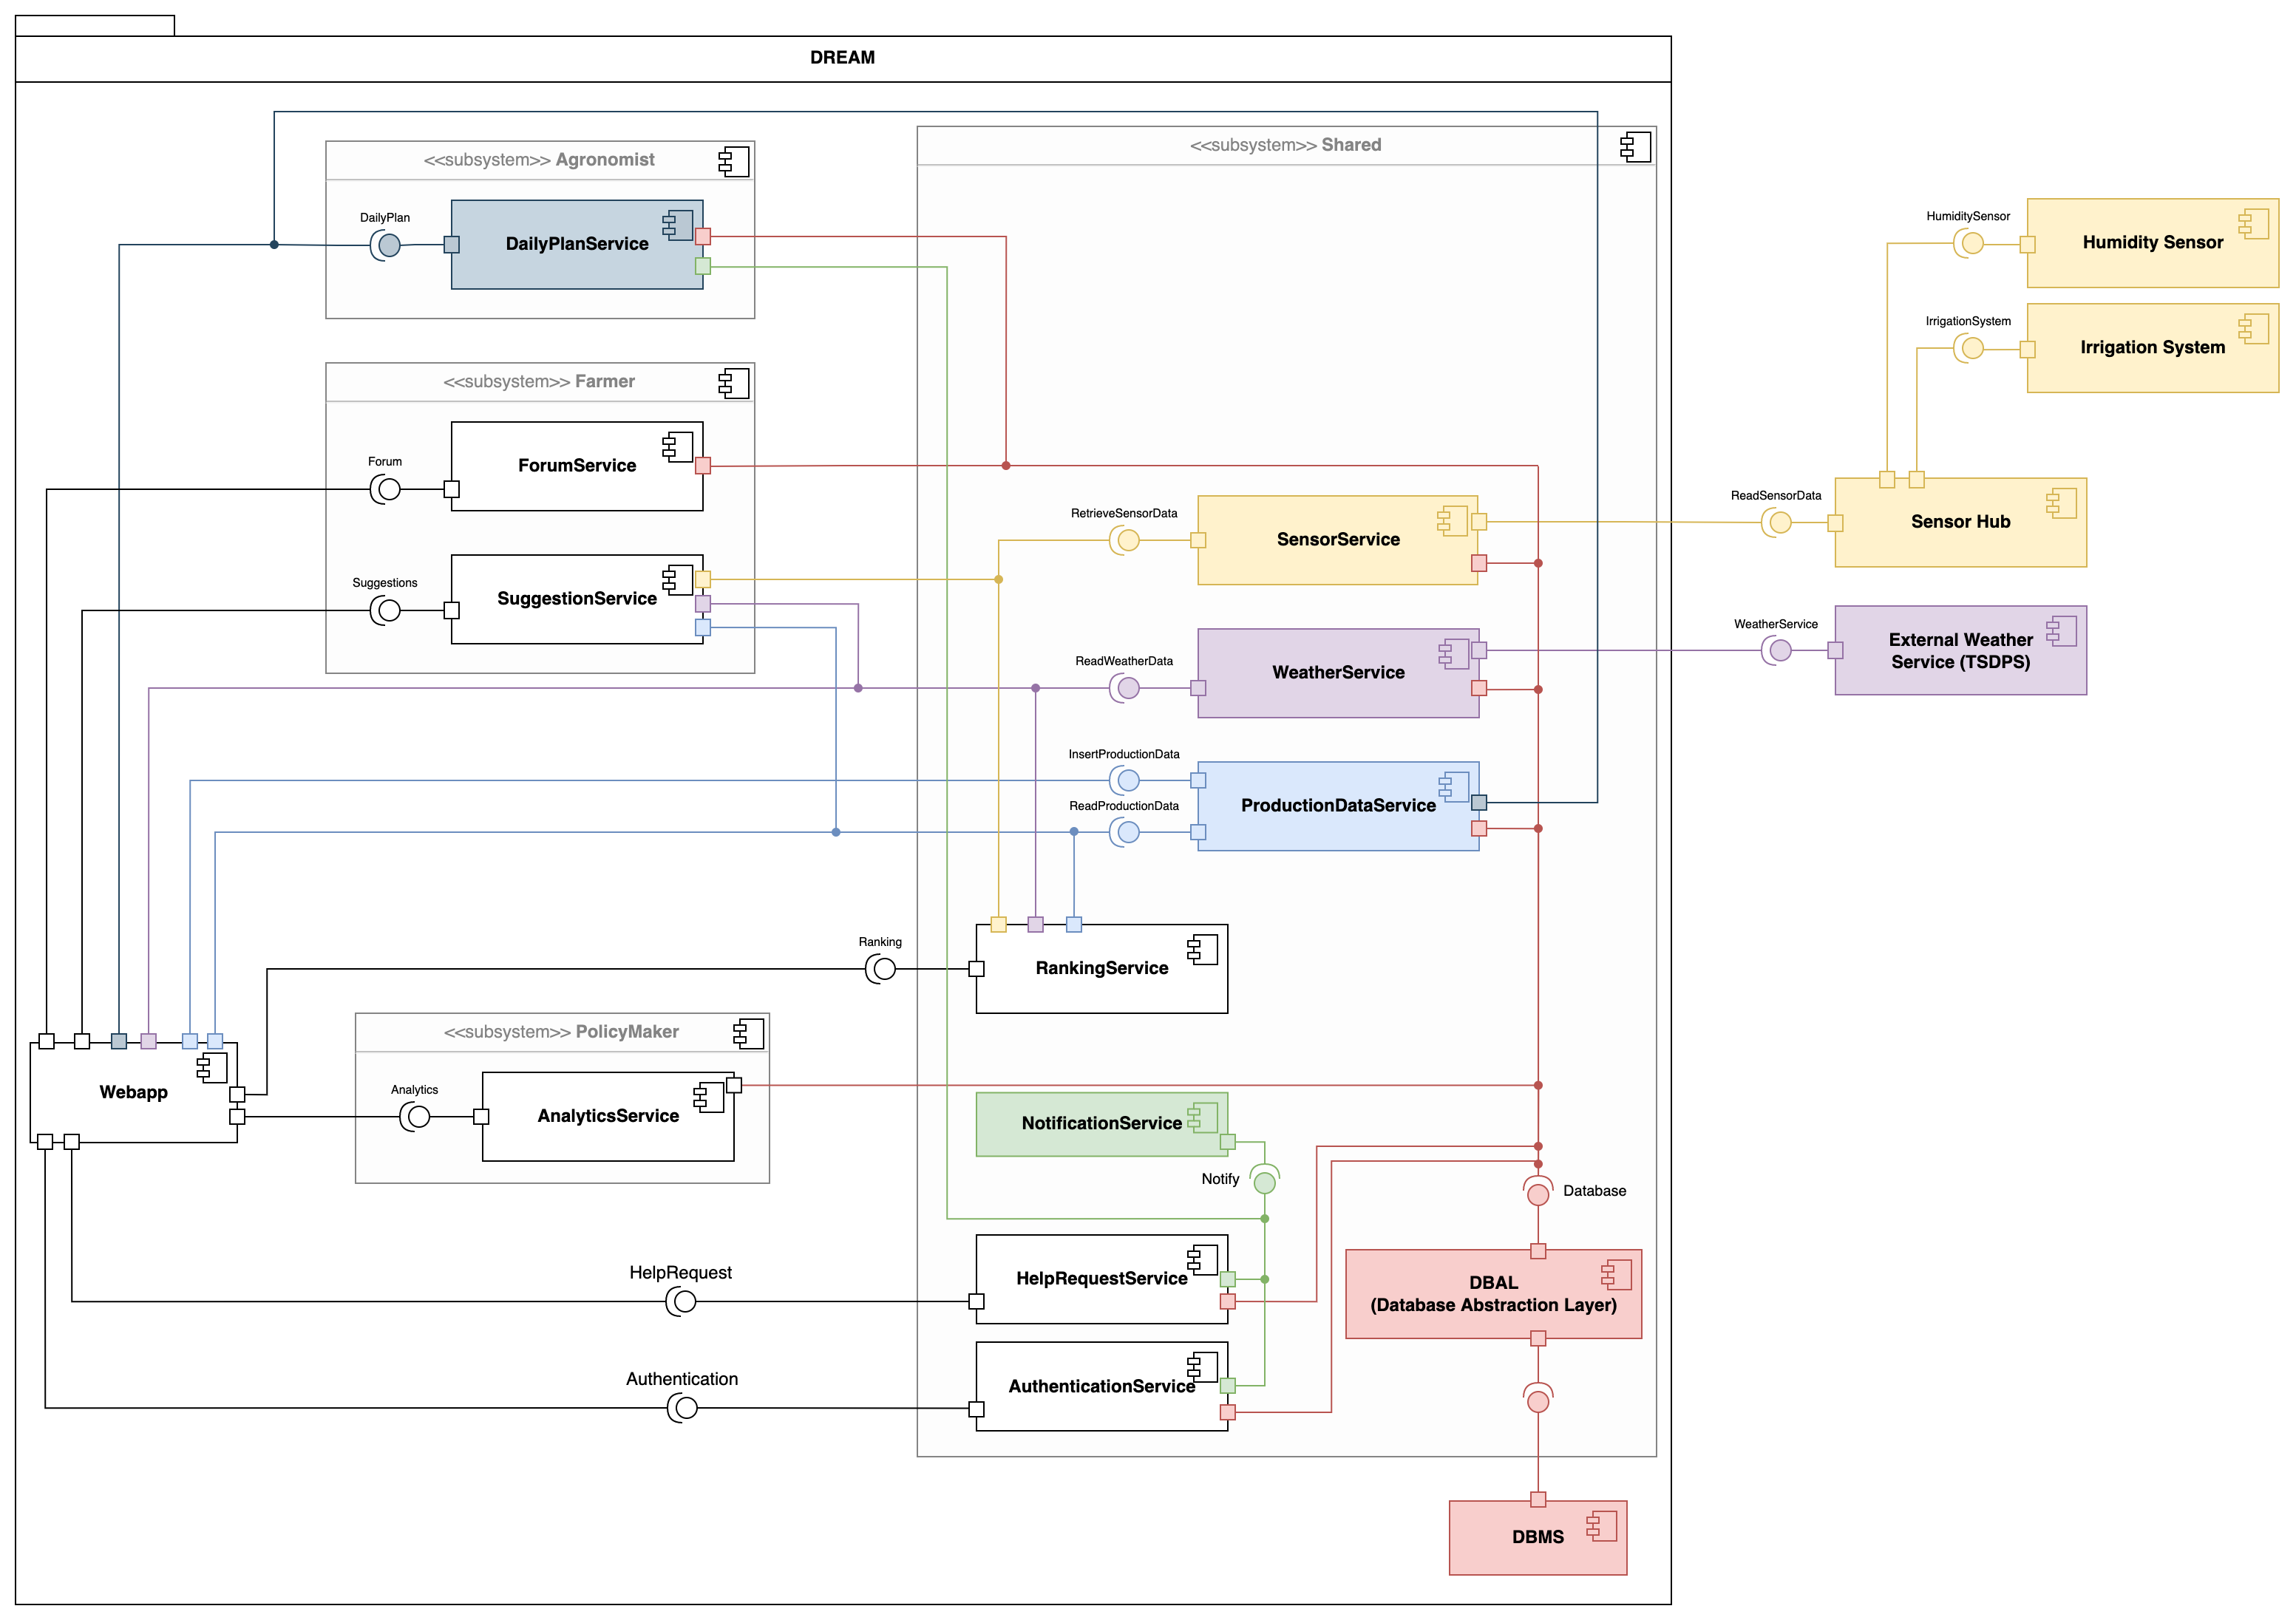
\includegraphics[width=16.5cm]{diagrams/components_diagram.png}
\subsection{Deployment view}
By the definition provided in "The Unified Modeling Language User Guide"\footnote{ISBN: 0-201-57168-4}, a deployment diagram is \textit{a diagram that shows the configuration of run time processing nodes and the components that live on them}. In other words, we represent the topology of processors and devices where our software executes.\\
The deployment diagram of \verb|DREAM| is the following:
\newpage
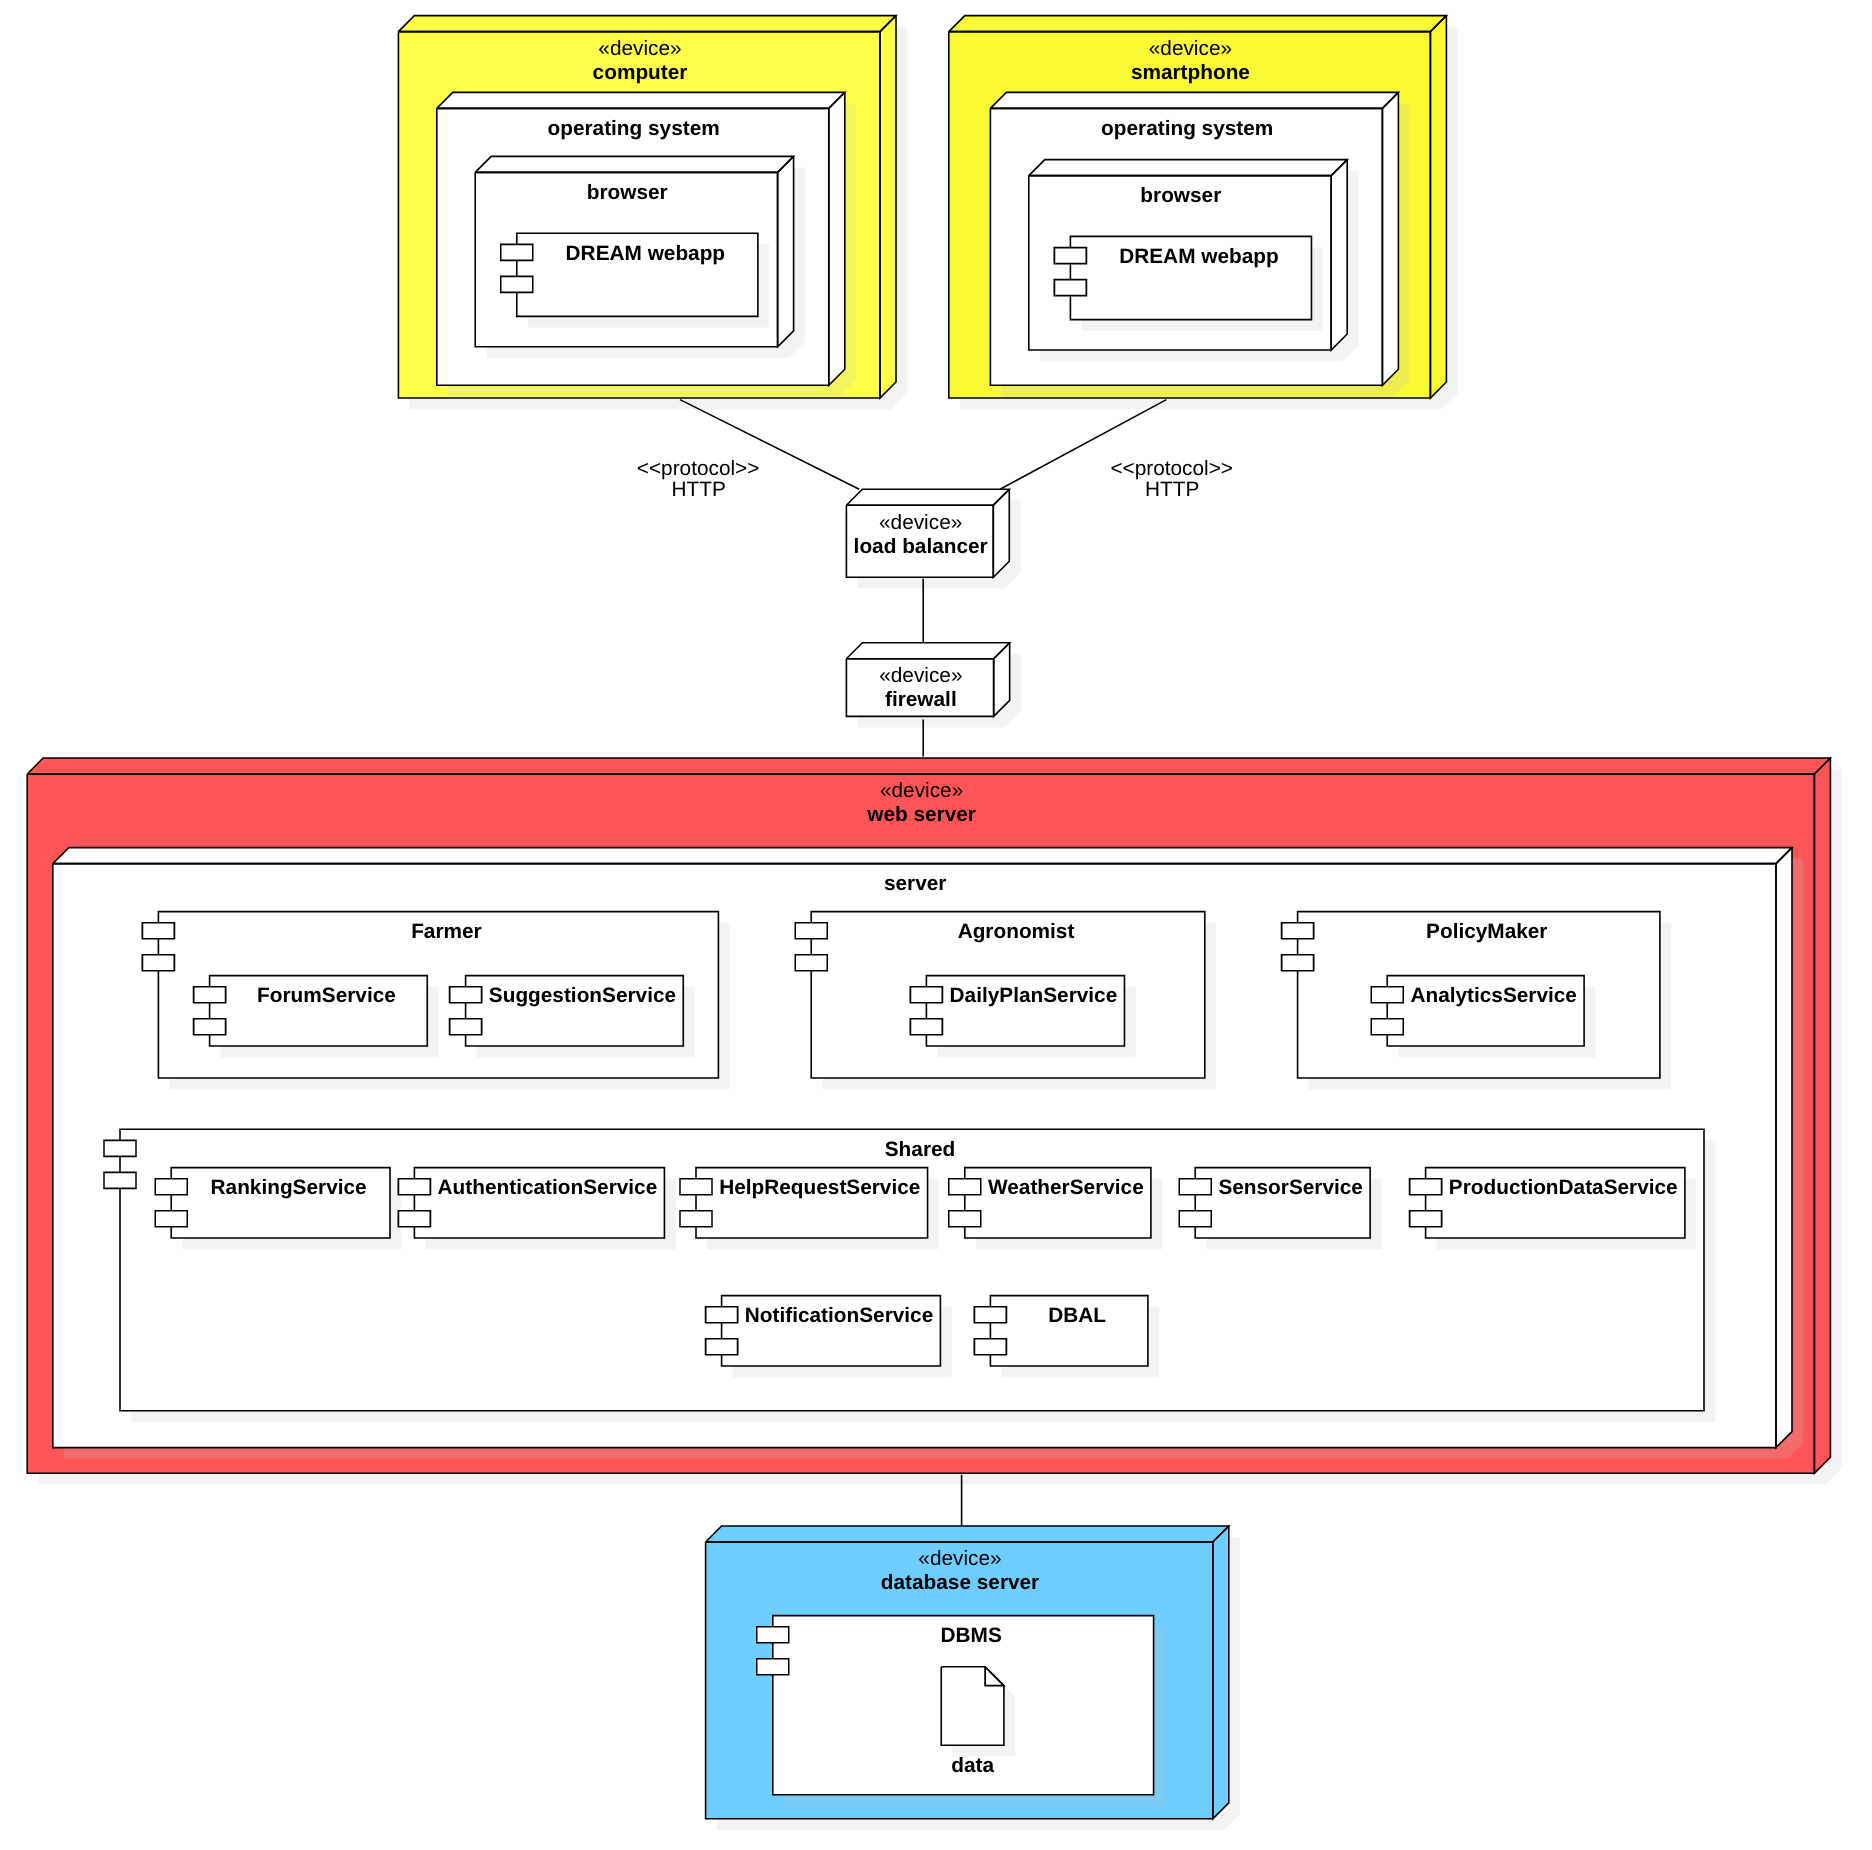
\includegraphics[trim=5cm 15cm 1cm 10cm,width=16.5cm]{diagrams/deployment_diagram.png}
\newpage
Some observations are required:
\begin{itemize}
    \item as previously specified, we opt for a 3-tiers architecture, with a web server that contains the whole business logic of the system and a database server with the data;
    \item some colours have been used for an easier visualization of the tiers;
    \item for the sake of simplicity, we have decided to represent only 2 possible clients, while the system is designed to support a much larger number;
    \item the number of web servers is more than one in order to offer faster responses and to scale better with more users;
    \item according to the amount of data to manage\footnote{see \textit{RASD - 3.3 Performance requirements} for an estimate of the storage capacity required.}, the data might be partitioned in more physical devices; for the sake of simplicity we have represented only one device since the access is hidden behind the DBAL;
    \item the architecture adopted for a scalable and secure routing of the users' requests to the servers is the FWLB (firewall load balancing), that is a \textit{deployment architecture where multiple firewall systems are placed behind Server Load Balancers}\footnote{\url{https://www.a10networks.com/blog/what-is-firewall-load-balancing-fwlb/}.}.
\end{itemize}
\subsection{Runtime view}
In this section the interactions among the components (identified at section \ref{Component view}) are shown. In order to make the presentation clearer, the UML notation of sequence diagrams is used.\\ It should be noticed that not all the use cases and scenarios identified in \textit{RASD - 3.2.3 Scenarios} and \textit{RASD - 3.2.4 Use cases} are represented here. We have decided to explicitly describe only the most relevant use cases, since in many occasions the interaction among the components is more or less the same. As a matter of fact, it often occurs that the difference lies only in the function invoked on a specific component; since all the interfaces are well-explained in the rest of this document (see section \ref{Component interfaces}), we opted to avoid this repetition.
Furthermore, the DBMS component is not represented in any sequence diagram because its interaction with the DBAL is hidden behind the software framework adopted.
\newpage
\begin{figure}[H]
   \centering
   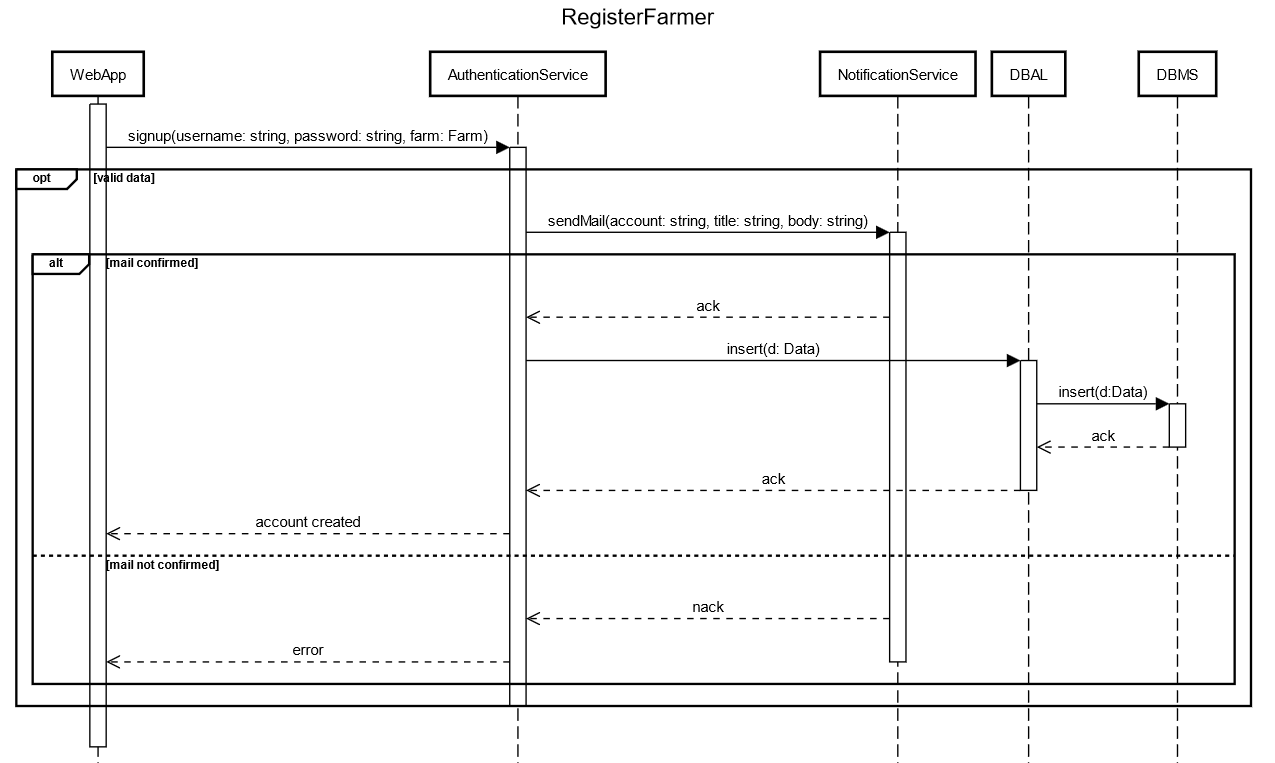
\includegraphics[scale=0.40]{diagrams/sequence diagrams/RegisterFarmer.png}
    \caption{Sequence diagram that describes the RegisterFarmer use case.}
\end{figure}
This sequence diagram describes the process of registration of a farmer in the system. The farmer invokes the signUp method on the AuthenticationService, which checks the validity of the data (length of the password, ...) and, in case data is valid, it exploits the NotificationService to send an e-mail to the farmer with a link to verify the account. In case the account is verified, the AuthenticationService stores the new account in the database and positively notifies the farmer, otherwise an error is sent.

\newpage
\begin{figure}[H]
   \centering
   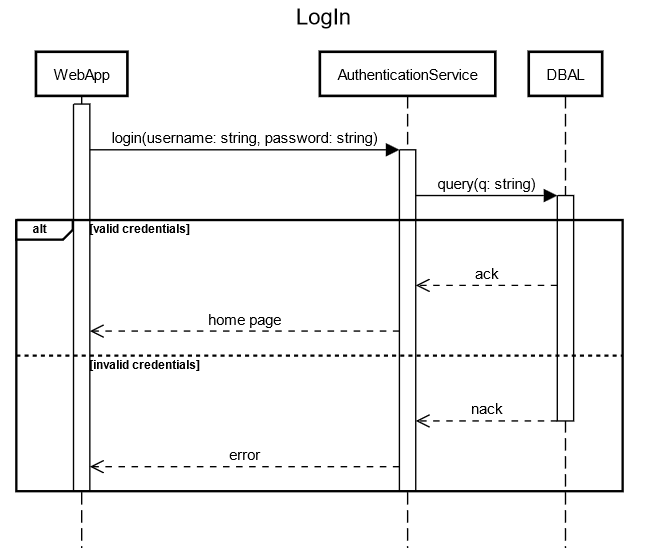
\includegraphics[scale=0.60]{diagrams/sequence diagrams/LogIn.png}
    \caption{Sequence diagram that describes the LogIn use case.}
\end{figure}

This sequence diagram describes how a user (farmer, agronomist or policy maker) can access to the system. The procedure is rather simple: the WebApp invokes the login method on the AuthenticationService which checks that the inserted credentials do not contain code for an SQL injection attack (in such a case, an error is returned to the WebApp; this branch is not represented in the diagram) and then queries the database (through the DBAL) to check whether a profile associated to the specified credentials actually exists. In such a case, the user logs in, otherwise he receives an error.\\
OBS.: from now on, checks on the data inserted by the user in order to avoid SQL injection attacks are not mentioned anymore, but they are present every time the user invokes methods of \verb|DREAM| passing arguments (since it is a functionality offered by the software framework adopted, it is not meaningful neither to represent nor to mention it every time).

\newpage
\begin{figure}[H]
   \centering
   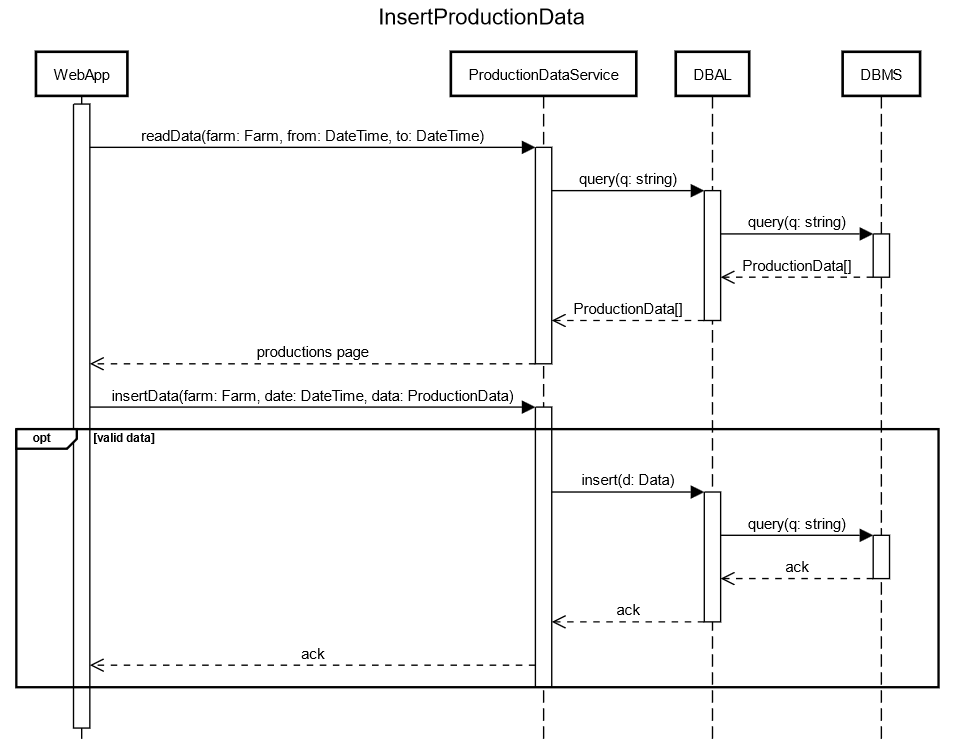
\includegraphics[scale=0.60]{diagrams/sequence diagrams/InsertProductionData.png}
    \caption{Sequence diagram that describes the InsertProductionData use case.}
\end{figure}
This sequence diagram describes the procedure through which a Farmer, starting from the home page, can insert production data in the system. According to the corresponding use case, the farmer automatically invokes the readData method when opening the "my productions" page. This call triggers an underlying retrieval of data from the database. Next, the Farmer calls insertData with all the details of the production to insert and, after a check about the validity, the data is inserted into the database and an ack is returned to the WebApp.

\newpage
\begin{figure}[H]
   \centering
   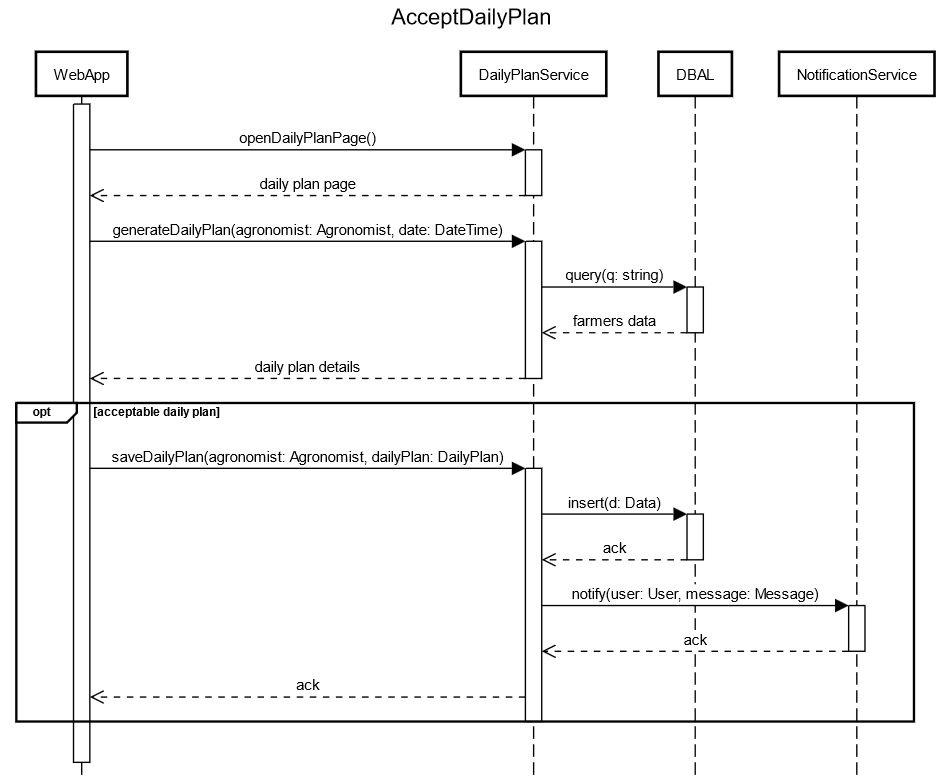
\includegraphics[scale=0.40]{diagrams/sequence diagrams/AcceptDailyPlan.png}
    \caption{Sequence diagram that describes the AcceptDailyPlan use case.}
\end{figure}
This sequence diagram describes the interactions that occur when an agronomist generates and accepts a new daily plan. First of all, the agronomist opens the daily plan page and then he selects the date of his next working day. The DailyPlanService queries the database to retrieve data about the Farmers that he needs to generate a suitable daily plan for the agronomist. In case the daily plan is acceptable to the agronomist, the WebApp invokes the saveDailyPlan method on the DailyPlanService, that stores the new daily plan in the database and then notifies the involved farmer (such interaction is not shown in the diagram).\\
OBS.: In order to modify the daily plan, specific methods are offered by the DailyPlanService. See section \ref{Component interfaces} for more details (sequence diagrams are omitted for the sake of simplicity).

\newpage
\begin{figure}[H]
   \centering
   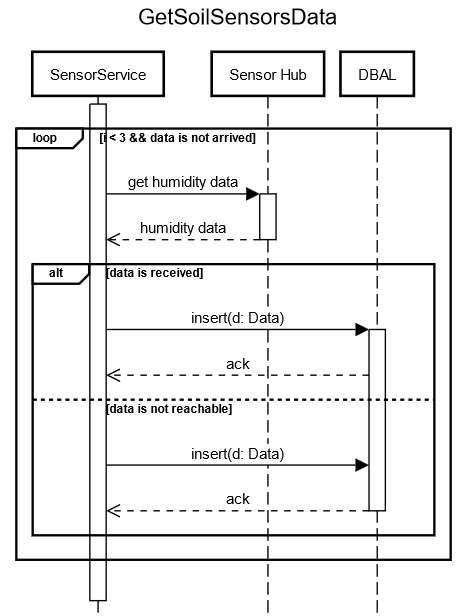
\includegraphics[scale=0.60]{diagrams/sequence diagrams/GetSoilSensorsData.png}
    \caption{Sequence diagram that describes the GetSoilSensorsData use case.}
\end{figure}
This sequence diagram describes the process with which \verb|DREAM| retrieves data from the humidity sensors (the process for the water irrigation system is analogue). Every time a timeout expires, the SensorService gets in contact with the Sensor Hub through its interface. If the data arrives, then such data is stored in the database, otherwise the SensorService stores in the database that at that specific timestamp the sensor was not reachable.

\newpage
\begin{figure}[H]
   \centering
   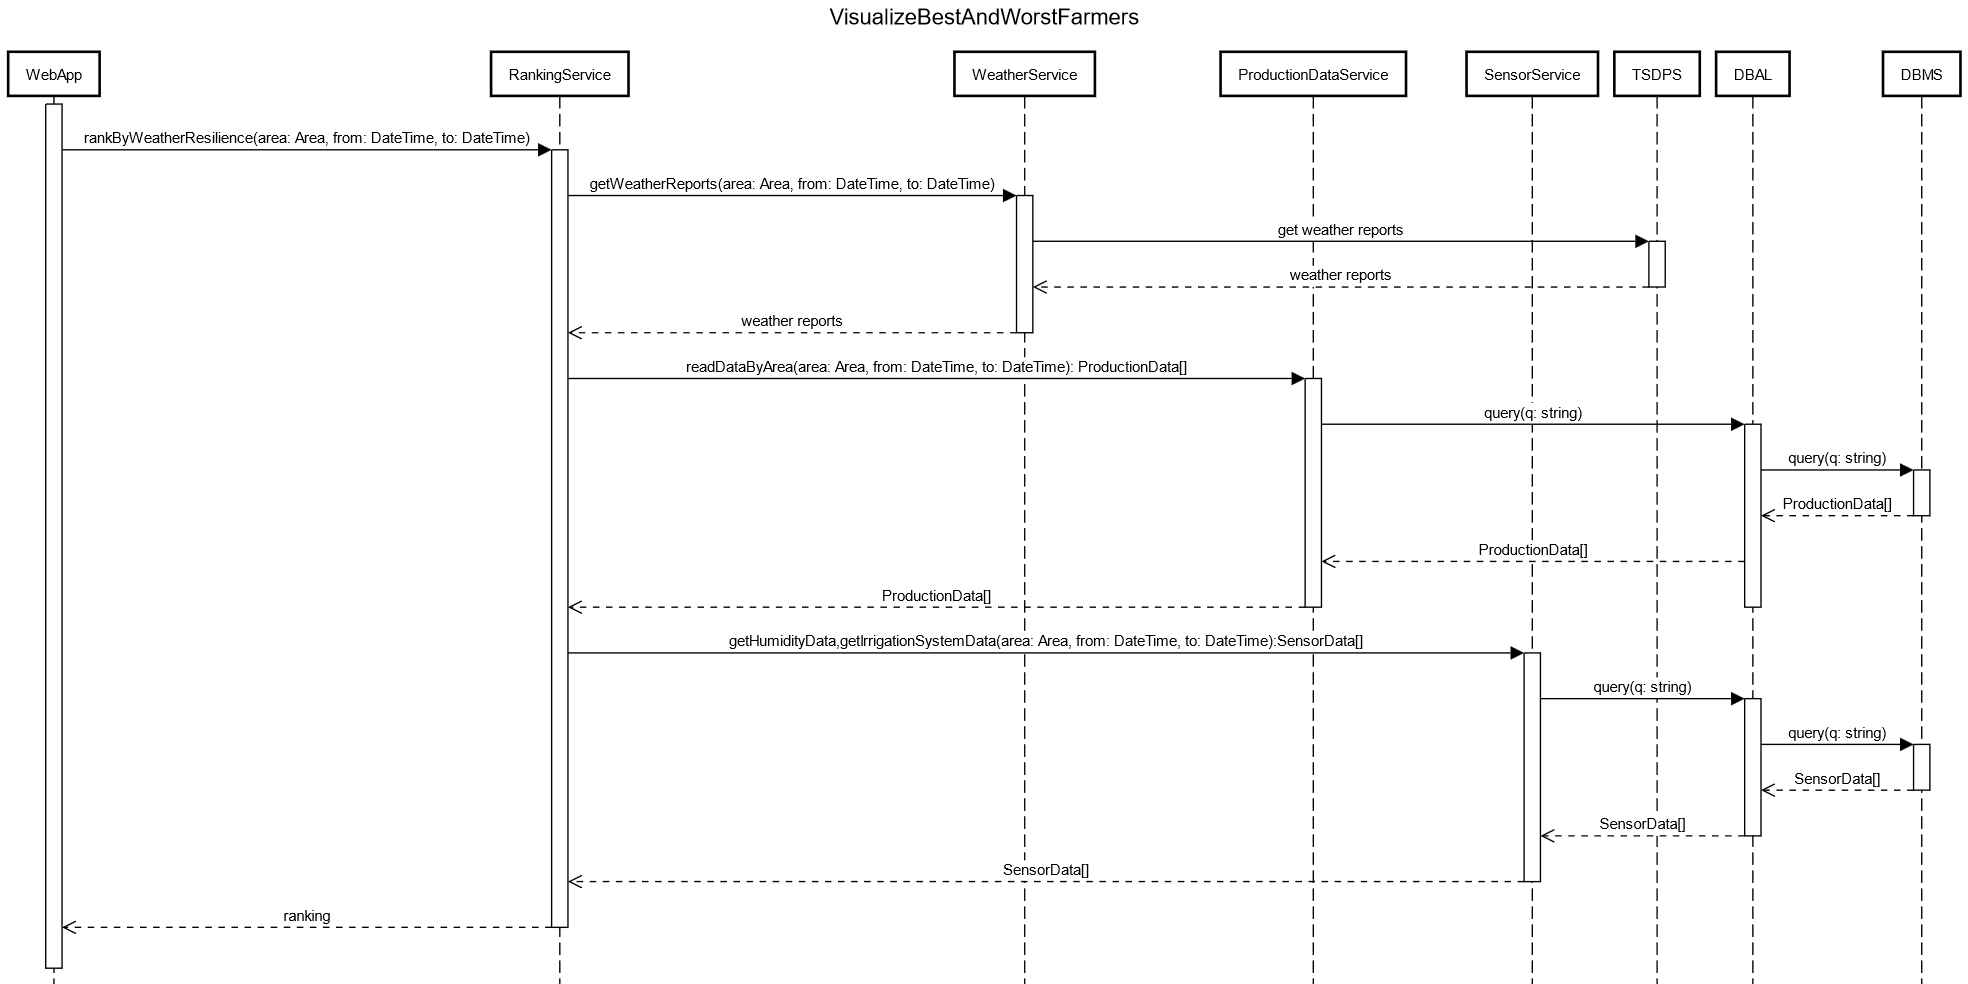
\includegraphics[scale=0.30]{diagrams/sequence diagrams/VisualizeBestAndWorstFarmers.png}
    \caption{Sequence diagram that describes the VisualizeBestAndWorstFarmers use case.}
\end{figure}
This sequence diagram describes the process that leads to the ranking of farmers. The policy maker invokes the rankByWeatherResilience method on the RankService, which exploits the WeatherService to retrieve the weather reports from the TSDPS; moreover, RankService queries the database to retrieve all the data about farmers it needs to rank them, and finally it provides the policy maker the ranking.

\newpage
\begin{figure}[H]
   \centering
   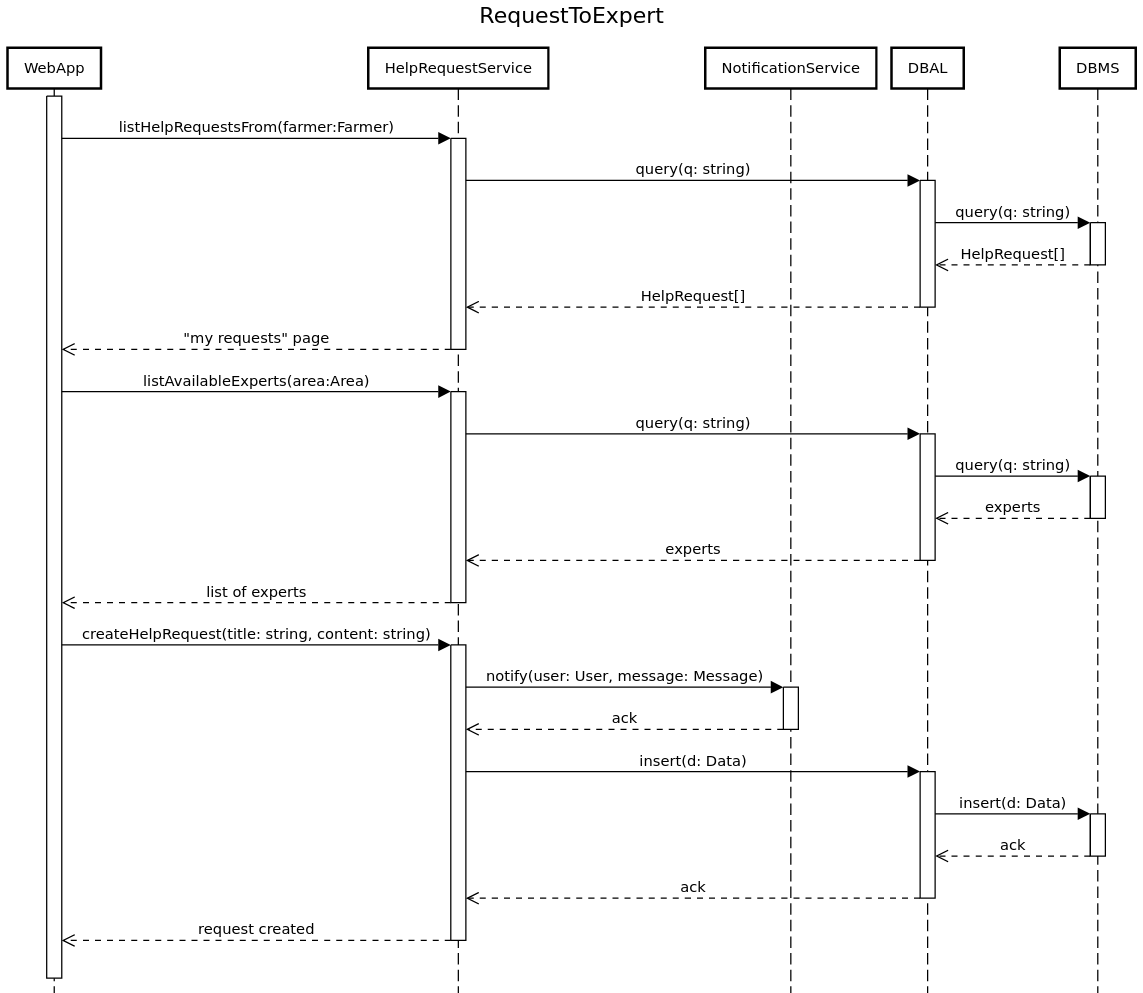
\includegraphics[scale=0.40]{diagrams/sequence diagrams/RequestToExpert.png}
    \caption{Sequence diagram that describes the RequestToExpert use case.}
\end{figure}
This sequence diagram represents the way a farmer can ask for help to an expert (agronomist or best-performing farmer). Starting from the home page, the farmer open the "my requests" page which implies a query to retrieve all the past requests of the farmer. Next, the farmer selects the expert from which he wants to receive some help and invokes the createHelpRequest method on the HelpRequestService. This service exploits the NotificationService to notify the expert, and, in case the the expert is already connected on Internet, an ack is received, the request is inserted in the database and the farmer is positively notified. It should be remarked that if the expert is not available, the system notifies the farmer that the expert will be notified as soon as he accesses \verb|DREAM| (this branch has been omitted for the sake of simplicity).

\newpage
\begin{figure}[H]
   \centering
   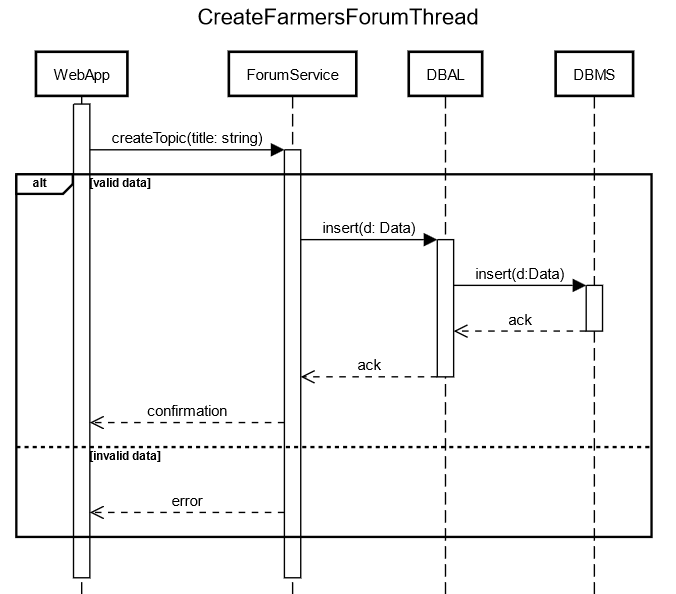
\includegraphics[scale=0.40]{diagrams/sequence diagrams/CreateFarmersForumThread.png}
    \caption{Sequence diagram that describes the CreateFarmersForumThread use case.}
\end{figure}
This diagram describes the process of creation of a new discussion thread by a farmer. It invokes the createTopic method on the HelpRequestService and, if the data inserted are valid, the service stores the information in the database and positively notifies the farmer, otherwise an error is shown.
\newpage
\subsection{Component interfaces}\label{Component interfaces}
\subsection{Selected architectural styles and patterns}
According to the definition provided by David Garlan and Mary Shaw\footnote{January 1994, CMUCS-
94-166, see "An Introduction to Software Architecture"
at \url{http://www.cs.cmu.edu/afs/cs/project/able/ftp/intro_softarch/intro_softarch.pdf}.}, \textit{an architectural style determines the vocabulary of components and connectors that can be used in instances of that style, together with a set of constraints on how they can be combined}.\\
\paragraph{Architectural style}
Given that the tasks that \verb|DREAM| has to achieve can be perfectly reached by implementing the system as a web application, and given that the most wide-spread, standardized and successful architectural style for distributed (web) applications is the client-server one, we have decided to opt for it. As a matter of fact, every time a user (farmer, agronomist or policy maker), namely a client, has to access the system, it sends a request to \verb|DREAM|, or better, to the server of \verb|DREAM|, which processes it and answers with a response. Moreover, our choice features 3 tiers with a thin client.\\
The main advantages of this choice related to the system we have to design are:
\begin{itemize}
    \item \textbf{scalability}: the number of resources can be easily increased when needed; thanks also to the decision of adopting a 3-tiers architecture, the data is apart from the business logic, therefore the storage capacity can be increased without affecting the anything else
    \item \textbf{accessibility}: the access to the system can be done with every possible device with a browser installed and from every location as long as an Internet connection is available. Despite this characteristic might not seem as important as the others identified in the \textit{RASD}, it is relevant because it provides much flexibility to the users: given their credentials, they can access from everywhere;
    \item \textbf{security}: users can access only through their credentials; this is a method for access controls and guarantees that only authorized users are granted access.
\end{itemize}
\subsection{Other design decisions}
\paragraph{Relational database}
We have decided to opt for a relational database because they perfectly match the use case of \verb|DREAM|. As a matter of fact, according to \textit{RASD - 3.3 Performance requirements}, there is not a huge number of relations between the entities of the data, thus a graph database would be counter-productive, because of its characteristic of being schema-less; the system has not strict time requirements, therefore adopting a key-value database would be uselessly expensive; the amount of data to manage is big, but not in the order required for matching the use case of a columnar database; finally, since data has to be pre-processed by \verb|DREAM| before reaching the users (in other words we accept data exiting the database at a low level), then we avoid a document-oriented database (also because it would make us waste a lot of space).
\paragraph{Database abstraction layer}
A DBAL is useful way to abstract from the details of the specific technology adopted for the database. It allows to reduce the amount of work required for the implementation of the components to manage the data because it provides APIs that hide the technicalities of the specific database chosen.
\paragraph{Model view controller}
The MVC is a software design pattern that allows to design a software application using 3 different main elements:
\begin{itemize}
    \item the model, which provides all the methods to access the data of the application;
    \item the view, which allows to visualize the data in the model and deals with the interaction between the system and the user;
    \item the controller, which receives the commands of the users and carries them out by modifying the state of the other two components.
\end{itemize}
The adoption of the MVC brings many advantages during the implementation phase of \verb|DREAM|. It allows to easily organize large-size web applications, to implement graphical interfaces with less effort, to easily doing planning and maintenance and many others.
\paragraph{Multi-page application}
....Christian or Chiara......
\paragraph{Thin client}
// to do
\paragraph{Algorithms}
.....Some remarkable algorithms.....
\section{User Interface design}
\section{Requirements traceability}
\section{Implementation, integration and test plan}
\section{Effort spent}
\section{References}
\end{document}
